\section{Design and Implementation}
\label{sec:implement}

\NM{} is designed as a drop-in replacement for the default memory allocator. It intercepts all memory allocation/deallocation APIs via the preloading mechanism. Therefore, there is no need to change the source code of applications to employ \NM{}, and there is no need to use the custom OS or hardware. 

Different from existing work, \NA{} aims to reduce remote accesses, and balance the workload among different hardware nodes. It also utilizes huge page support to improve the performance, and designs its interleaved and block-wise memory allocation to accommodate shared objects. Multiple components that differentiate it from existing allocators are discussed in the remainder of this section. 
  
\NA{} also borrows many known mechanisms of existing allocators. First, it utilizes the size class to manage objects. Instead of allocating the exact size, \NA{} will round the size of an allocation to its closest size class. Similar to TcMalloc~\cite{tcmalloc}, \NA{} also utilizes fine-grained size classes for small objects, such as 16 bytes apart for objects less than 128 bytes, and 32 bytes apart for objects between 128 bytes and 256 bytes, then power-of-2 sizes afterwards. Second, it utilizes the ``\textbf{Bi}g-\textbf{B}ag-\textbf{o}f-\textbf{P}ages'' mechanism that all objects in the same bag will have the same size class, and separates the metadata from actual objects. \NA{} only tracks the size information of each page, which helps reduce its memory overhead for the metadata. Third, \NA{} utilizes freelist to manage freed objects. Every freed object will be added into a corresponding freelist, and objects in the freelist will be allocated first in order to reduce possible cache misses. Further, \NA{} utilizes the first word of freed objects to link different objects, which is similar to Linux and TcMalloc~\cite{tcmalloc}. This mechanism helps to reduce the memory overhead, but is prone to memory vulnerabilities, such as buffer overflows and double-frees~\cite{DieHarder, Guarder}.     

\begin{figure*}[h]
\begin{center}
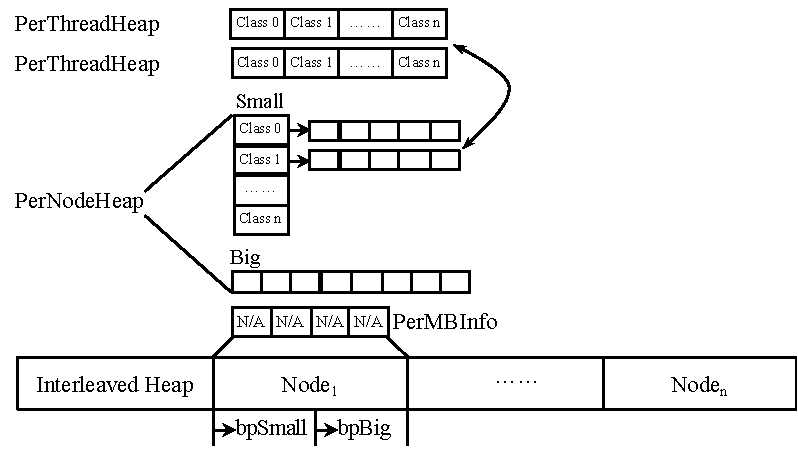
\includegraphics[width=0.8\textwidth]{figure/heaplayout1}
%\includegraphics{figure/overview2}
\end{center}
\vspace{-0.1in}
\caption{Overview of \NA{}.
\label{fig:overview}}
\vspace{-0.1in}
\end{figure*}

\subsection{Topology Aware Task Assignment} 
\label{sec:taskassign}

Existing allocators typically do not schedule tasks explicitly, but relying on the default OS scheduler. The OS scheduler performs very well for the UMA architecture, since the latency of accessing the memory controller is the same for every core. However, the NUMA architecture imposes additional challenge~\cite{Majo:2015:LPC:2688500.2688509}. If a task is moved to a new node, it has to access all of its memory through the interconnect, resulting in a higher memory latency. The scheduling may lead to significant performance difference for memory-intensive applications. Therefore, typically tasks are bound to a specific core/processor for the NUMA architecture~\cite{terboven2012assessing, terboven2012task, Majo:2015:LPC:2688500.2688509}.  

%Similarly, \NA{} embeds the task assignment into its memory management. 
Due to the importance of task assignment to  memory locality, \textit{\NA{} embeds a topology-aware task assignment, which makes it different from existing allocators}. Every thread is bound to a specific node, where its memory allocations will be based on the location of its task, as described in Section~\ref{sec:nodeaware-memory}. To balance the workload of each node, \NA{} utilizes a round-robin manner on the nodes to assign the tasks , which is similar to TBB-NUMA~\cite{Majo:2015:LPC:2688500.2688509}. Basically, a newly-created thread will be assigned to a node that is different from its preceding and subsequent sibling. This ensures that each processor/node will have a similar number of threads, and therefore a similar workload. An alternative approach is to assign the same number of threads as cores to one node, and then assign subsequent threads to the next node. However, this approach has two issues. First, it may cause significant performance issue for applications with the pipeline model due to remote accesses, if threads of different stages are assigned to different memory nodes. Second, it may not fully utilize all memory controllers, if the number of threads is less than the number of cores in total.    

In the implementation, \NA{} recognizes the hardware topology via the \texttt{numa\_node\_to\_cpus} API, which tells the relationship between each CPU core and each memory node. It intercepts all thread creations in order to bind a newly-created thread to a specific node. \NA{} employs \texttt{pthread\_attr\_setaffinity\_np} to set the attributes of a thread, and passes the attribute to its thread creation function. Therefore, every thread is scheduled to the specified node upon the creation time. Note that a thread is pinned to a node in \NM{}, instead of a core, which still allows the OS scheduler to perform the load balance when necessarily. 

\subsection{Node-Aware Memory Management} 
\label{sec:nodeaware-memory}

\NA{} designs a node-aware memory management based on its task assignment. All heap objects of a thread will be \textit{physically} allocated from the node that the thread is currently pinned to, unless otherwise stated (Section~\ref{sec:mainthread}). Since a memory allocator only deals with virtual memory, but not physical memory, \textit{\NA{} binds every range of its virtual memory to a particular node via the \texttt{mbind} system call}. Therefore, \NA{} is able to identify the physical node information based on a virtual address, which is the same as existing work~\cite{tcmallocnew}. However, \NA{} manages memory allocations and deallocations differently, which explains its significant performance advantage over the existing work~\cite{tcmallocnew} (see Section~\ref{}). 

\NA{} handles deallocations of objects carefully, in order to ensure node-aware memory allocations. \NA{} utilizes different mechanisms to handle large objects and small objects. In \NM{}, an object with the size larger than 512KB will be treated as a big object. Otherwise, it is belonging to a small object. As described above, \NM{} maintains multiple size classes for small objects. Upon each deallocation, \NA{} determines its physical node (based on its virtual address) and the size information in order to place it correspondingly. For small objects, if an object is allocated from a different node, it will be placed into the common freelist of that node. Otherwise, it will be placed into the freelist of the deallocation thread. Utilizing a per-thread list avoids the synchronization overhead, since only one thread is allowed to access its per-thread list. 
Big objects are handled differently due to two reasons. First, an application typically has relatively fewer number of big objects. Therefore, it is expensive to maintain size classes for big objects. Second, every big object has a larger impact on the memory consumption, which should be re-utilized as soon as possible. Therefore, each node keeps a per-node freelist to track big objects in the current node. Different from existing allocators, big objects are not returned to the OS immediately upon deallocations~\cite{Hoard, tcmalloc}, which reduces cache loading operations and memory management overhead of the OS.  Instead, they will be tracked in the per-node freelist, and will be utilized to satisfy future allocation requests of both big objects and small objects. Upon the deallocation of a big object, \NM{} tries to coalesce with its previous and next neighbor, if its neighbor is also freed.  
 
\NA{} manages memory allocations as follows. Basically, an allocation will be satisfied from the corresponding freelist at first, if some freed objects exist. Otherwise, a new/never-used object will be allocated.  Objects in the freelist will be allocated using the last-in-first-out order, which helps reduce possible cache misses since last-freed objects are more likely to be hot. A big object will be allocated from the per-node freelist, while a small object will be allocated from the thread's per-thread list if possible and then the per-node freelist. \NM{} moves small objects between per-thread lists and per-node lists: if freed objects in a per-thread list is over a pre-defined threshold, a percentage of freed objects will be moved to the thread's per-node list; Whenever the per-thread list is empty, some objects will be moved from the corresponding per-node freelist. Both movement will take an adaptive mechanism. For instance, if a per-thread list keeps migrating objects from its per-node list successfully, then the percentage of moving to per-node list will be reduced. Similarly, if a per-node list do not have objects to move to the per-thread list, \NM{} will move less frequently.  

In its implementation, \NA{} reduces the overhead of frequent system calls, and borrows the information-computable design from existing allocators in order to quickly locate the physical node information~\cite{FreeGuard, Guarder}. The basic idea of its memory layout is illustrated in Fig.~\ref{fig:overview}. Basically, \NA{} takes the advantage of the huge address space of 64-bits machine to achieve the quick lookup. Instead of frequently allocating the memory from the OS, \NA{} obtains a big chunk of memory (few terabytes) from the underlying OS initially, and then divides it to multiple chunks with the same size, where each chunk will be bound to a specific memory node as illustrated in Fig.~\ref{fig:overview}. Therefore, the physical node information could be computed directly from the virtual address, by checking the distance from the starting address of the heap. Comparing the method of using a hash table to track the node information~\cite{tcmallocnew}, this mechanism is much faster, since it avoids the hashing and lookup overhead.  

Each chunk belonging to one node is further divided into two parts, one for small objects (managed with the \texttt{bpSmall} bump pointer) and one for big objects (managed using the \texttt{bpBig} pointer). There are two reasons to separate them. First, we plan to utilize huge page support for big objects, but not small objects, which is further described in Section~\ref{sec:hugepage}.  Second, placing big objects together helps to coalesce two continuous objects into one bigger object. For small objects, \NM{} employs the ``\textbf{Bi}g-\textbf{B}ag-\textbf{O}f-\textbf{P}ages'' (BiBOP) style that each bag will have multiple continuous pages, and each bag will have objects with the same size class. \NM{} currently sets its bag size of small objects to be one megabytes. An object with the size larger than 512 kilobytes is considered to be a big object, which will be always aligned to megabytes. Therefore, \NM{} only requires to record the size information for each megabytes, shown as \texttt{PerMBInfo} in Fig.~\ref{fig:overview}. \NM{} embeds the availability information of each chunk to the \texttt{PerMBInfo} structure, using the lowest significant bit of the size. Each node has  a per-node heap, which includes a per-node freelist to track big objects, and multiple freelists to track small objects with different size classes. As described above, each thread also has its freelists for different size classes. Small objects can be moved between a per-thread freelist and a per-node list as described above. 
 

%When a big object is freed, \NM{} checks the availability of its previous and next neighbor, and performs the coalesce if its neighbor is also available. \NM{} re-utilize a freed big object for a bag of small objects, since the bag size of small objects and big objects are both aligned to one megabytes. This is different from most existing allocators, which typically returns big objects to the OS upon deallocation. Comparing to them, \NM{} reduces cache misses by re-utilizing big objects.  

\paragraph{Cache Warmup Mechanism} For small objects, \NM{} also borrows the cache warmup mechanism of TcMalloc~\cite{tcmalloc}. TcMalloc utilizes the \texttt{mmap} system call to obtain multiple pages (depending on the class size) from the OS each time, when it is running out of the memory for one size class. For such a memory block, TcMalloc adds all objects of this block into the freelist at one time. Since TcMalloc utilizes the first word of each object as the pointer for the freelist, this mechanism warms up the cache by referencing the first word of each object during the adding operation. According to our observation, this warmup mechanism improves the performance of one application (\texttt{raytrace}) by 10\%. Based on our understanding, the performance improvement is caused by data prefetches, since adding objects to the freelist has a simple and predictable pattern. \NM{} employs a similar mechanism for small objects with the size less than 256 bytes, and adds all objects inside a page to the freelist. A bump pointer is used to track the position of never-used objects, whose updates do not require to be exactly one page each time. By comparison, TcMalloc may waste some memory in the end of each block, if the block size is not equal to multiple times of the class size.   

\subsection{Interleaved Heap} 
\label{sec:mainthread}

\NA{} proposed a new interleaved  heap for shared objects. Based on our observation, most NUMA performances issues identified by existing NUMA profilers are related to shared objects~\cite{XULIU, MemProf}. Shared objects are typically allocated in the main thread, but are accessed concurrently by multiple children threads later. Allocating the physical memory for shared objects in one node may introduce load imbalance issue, and therefore causing significant number of remote accesses. Therefore, \NA{} reserves a range of memory for shared objects, called as ``Interleaved Heap'' in Fig.~\ref{fig:overview}. \NA{} utilizes the \texttt{mbind} system call to specify that the physical pages of this range will be allocated from all nodes interleavedly. This design helps balance the volume of memory accesses of all memory controllers, reducing interconnect congestion and load imbalance. 

\begin{comment}
\begin{wrapfigure}{r}{0.6\textwidth}
\centering
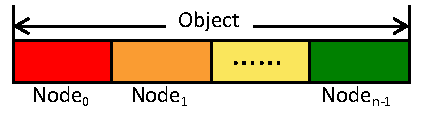
\includegraphics[width=3in]{figure/blockwise}
\vspace{-0.1in}
\caption{Block-wise Memory Allocation\label{fig:blockwise}}
\vspace{-0.1in}
\end{wrapfigure}
\end{comment}

\NA{} allocates the memory in a block-wise way for shared objects, when the size of an allocation is larger than the twice of the multiplication of nodes and the page size. The basic idea of block-wise allocation is illustrated in Fig.~\ref{fig:blockwise}. The key reason to use the block-wise allocation is that children threads may access the memory continuously~\cite{XULIU}. In addition to that, the block-wise allocation will still maintain the balance between different memory nodes, which won't cause unnecessary performance issue. 
 
During the implementation, \NA{} only allocates shared objects from the main thread in the interleaved heap. Although it may benefit the performance if shared objects allocated in children threads are also using the interleaved heap, especially for applications with the pipeline model, the overhead of tracking shared objects is typically larger than the performance benefit based on our evaluation. 

It is very important to identify shared objects correctly. Otherwise, it will introduce performance issue by allocating private objects in a different node, causing remote accesses unnecessarily. \NA{} utilizes the allocation/deallocation pattern to identify shared objects: an object is treated as a shared one initially, and is allocated from the interleaved heap; If a newly-allocated object is deallocated before creating children threads, all objects from the corresponding callsite are considered to be private objects. Therefore, \NA{} utilizes the callsite to differentiate objects, which is determined by the program logic.  

However, it is very challenging to determine the allocation callsite \textit{uniquely} and \textit{efficiently} due to multiple reasons. First, function pointers are removed in most applications if they were compiled with an optimization, which makes it impossible to obtain return addresses (and callsite) via built-in functions. Second, applications have a wrapper for memory allocations, which requires multiple levels of call stacks to uniquely identify one callsite. Although there exist mechanisms to encode calling context explicitly~\cite{DBLP:conf/icse/SumnerZWZ10, DBLP:conf/cgo/ZengR0AJ014}, they require the recompilation of the applications. The \texttt{backtrace} function can obtain the callsite, but it is too slow to be used in production environment.

\NA{} proposes to utilize the sum of the stack position and the return address of the allocation to identify a callsite, called ``\textit{callsite key}''.  When memory allocations are invoked in different functions, their stack positions are likely to be different. The return address (of the application) tells the invocation placement inside the same function. However, this design cannot completely avoid mis-identification issue when there exists the allocation wrapper, where multiple allocations inside the same function will be treated as the same callsite. A shared callsite can be treated as a private callsite, if an object from  these callsites invokes the deallocation before creating children threads. For the performance reason, \NA{} obtains the return address quickly via a constant offset, where the offset is uniquely determined after the compilation of \NA{}. 

\NA{} utilizes a hash table to track the status of every callsite. Upon every allocation of the main thread, \NA{} checks the status of the allocation callsite, with the callsite key as described above. If the callsite key is not existing in the hash table or the callsite is identified as a shared callsite, the current allocation will be satisfied from the interleaved heap. Otherwise, it will be allocated from the per-node heap. When an allocation is satisfied in the callsite and the callsite is new, the corresponding allocation will be tracked in the second hash table. The second hash table will be checked upon deallocations, where the corresponding allocation callsite will be marked as private if an object is allocated in the same epoch. 

\subsection{Automatic Huge Page Support} 
\label{sec:hugepage}

\NA{} employs the existing huge page support to further improve the performance. Modern hardware typically installs with huge page support. A huge page is a page that its page size is much larger than 4 kilobytes. Currently, the Linux system has two page sizes, 4 kilobytes and 2 megabytes. Based on the existing study~\cite{hugepages}, huge pages can reduce Translation Look-aside Buffer (TLB) misses that may significantly affect the performance, since a huge page covers a larger range of memory than a normal page. Reducing TLB misses helps reduce the interferences on the cache utilization caused by TLB misses, and therefore reduces cache misses. Huge pages could also reduces the contention in the OS memory manager. We observed around 10\% performance improvement for some applications, when we are using huge page support. 

However, the default huge page support is not good for the performance~\cite{Gaud:2014:LPM:2643634.2643659, DBLP:conf/asplos/PanwarBG19}. In fact, it may have some harmful impact on the performance of NUMA systems. First, it can cause the \textit{hot page effect} when multiple frequently-accessed objects  were  mapped  to  the  same  physical  page, causing the overloading of the corresponding memory node. Second, huge pages are more prone to \textit{page-level false sharing}, when multiple threads are accessing different data inside the same page. Besides that, the huge page may increase the memory footprint~\cite{DBLP:conf/asplos/MaasAIJMR20}, if a partial range of a huge page is not accessed. 

\NA{} utilizes huge pages differently. Ideally, if huge pages are utilized for private objects, then there are no hot page effect and page-level false sharing. Also, if huge pages are only utilized for big objects or all small objects in a huge page will be allocated, then the memory footprint can be minimized. \NA{} takes these consideration into account. Each per-node heap is further divided into two parts as illustrated in Fig.~\ref{fig:overview}: small objects will be allocated from the first half and will be allocated using small pages, while big objects will be allocated from the second half with huge pages (2MB). When a big object is utilized for small objects, only frequently-allocated small objects can utilize such an object. We believe that our design balances the performance and memory consumption.   

\subsection{Efficient Objects Migration} 

\NM{} maintains per-thread heap and per-node heap in order to reduce the synchronization overhead, which indicates the necessity of moving objects between different heaps. All threads bounded to the same node will share the per-node heap. When a per-thread list has too many objects, some of them should be moved to the per-node list so that other threads could re-utilize these freed objects, reducing the memory consumption. Similarly, each per-thread list may need to obtain freed objects from its per-node heap, when a thread is running out the memory. These frequent migrations require an efficient mechanism. Currently, \NM{} utilizes singly link lists to manage freed objects, imposing an additional challenge of migrating objects efficiently. 

One straightforward method is to traverse the whole list to collect a batch of objects, and then moves them at a time. Although the idea of using the batch reduces the contention, but this still has multiple issues. First, traversing a list will actually pollute the cache of the current thread, especially when a thread is moving out objects from its per-thread heap. That is, the thread does not need to access these objects any more, where traversing these objects will bring these objects to the cache. Second, it is very slow to traverse a list, which may create thread contention when multiple threads are migrating freed objects from the per-node heap concurrently. We observed a 20\% slowdown for some applications due to this straightforward mechanism. \NM{} further proposes multiple mechanisms to migrate objects efficiently. 

\begin{wrapfigure}{r}{0.6\textwidth}
\centering
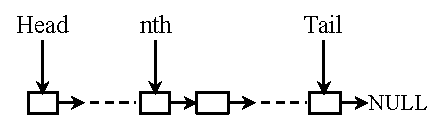
\includegraphics[width=3in]{figure/perthreadlist}
\vspace{-0.1in}
\caption{Avoiding the traverse of per-thread freelist\label{fig:perthreadlist}}
\vspace{-0.1in}
\end{wrapfigure}
In order to avoid the pollution on the per-thread cache in moving out objects, each per-thread freelist maintains two pointers that pointing to the least recent object (shown as the \texttt{Tail} object) and the $nth$ object separately, as shown in Figure~\ref{fig:perthreadlist}. Therefore, if a thread is going to migrate $n$ objects (between $(n-1)th$ and the \texttt{Tail} object), it only requires a forward check to obtain the pointer of $(n-1)th$ object and then it could move out $n$ objects at a time. After the migration,  the \texttt{Tail} pointer can be set to the original $nth$ object. But this mechanism alone cannot reduce the contention when multiple threads are concurrently obtaining objects.

\begin{wrapfigure}{r}{0.6\textwidth}
\centering
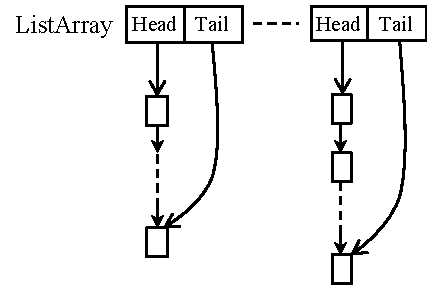
\includegraphics[width=3in]{figure/listarray}
\vspace{-0.1in}
\caption{An array of freelists for per-node heap\label{fig:listarray}}
\vspace{-0.1in}
\end{wrapfigure}
In order to avoid the bottleneck of the per-node heap, \NM{} introduces a circular array of freelists as shown in Figure~\ref{fig:listarray}, where the number of entries is a variable that can be changed by the compilation flag. This array has two pointers, one is \texttt{toGetIndex} and the other one is \texttt{toPutIndex}. When a thread migrates freed objects to the per-node heap, it will add the list of objects to the freelist pointed by \texttt{toPutIndex}, and update the index after the migration. Similarly, if a thread tries to obtain freed objects from the per-node heap, it will obtain all objects in the freelist pointed by the \texttt{toGetIndex}, and update the index afterwards. If the freelist pointed by the \texttt{toGetIndex} has no freed objects, indicating that there is no freed objects in the per-node heap for this size class, then the index is not updated. As described above, if a thread running on the other node just deallocates an object to the per-node heap, then this object will be added to the head of the freelist pointed by  \texttt{toPutIndex}, but the index is not changed after the deallocation.  
 

\subsection{Other Mechanisms}

\paragraph{Node-Local Metadata:} \NM{} guarantees that all of the metadata is always allocated in the same node, based on its task binding as described in Section~\ref{sec:taskassign}. Such metadata includes the PerMBInfo, per-node and per-thread freelists for different size classes, and freelists for big objects. \NM{} utilizes the \texttt{mbind} system call to bind a range of memory to a specific node.  

\paragraph{Memory Reutilization:} Some applications may create new threads after some threads have exited. \NM{} re-utilizes the memory for these exited threads. Basically, \NM{} introduces a thread index for each thread, which is utilized to index the corresponding per-thread heap.  \NM{} intercepts thread joins and cancels so that it can assign the indexes of exited threads for newly-created threads, and re-utilize their heaps correspondingly.  


\paragraph{MiniBag Design to Reduce Memory Consumption:} During the development, we noticed that excessive memory consumption  can be imposed when the OS utilizes huge pages by default, such as Machine B. In order to avoid this issue, we propose the combination of per-node heap and per-thread cache. \todo{In order to reduce the contention, \NM{} will obtain multiple objects at a time from the per-node heap. }

 
%https://queue.acm.org/detail.cfm?id=2852078

